\documentclass[12pt]{article}
\usepackage[utf8]{inputenc}
\usepackage[spanish]{babel}
\usepackage{geometry}
\usepackage{graphicx}
\usepackage{hyperref}
\geometry{a4paper, margin=1in}
\usepackage{enumitem}
\setlist{nosep}
\usepackage{booktabs}
\usepackage{array}


\title{Actividad 2: Sistema solar a escala en el campus}
\author{Astronomía para Todos \\ Grupo 2 - 2024-2}
\date{}

\begin{document}

\maketitle

\section*{Objetivo}

Construir un sistema solar a escala, en el cual el Sol tiene un tamaño de un balón de baloncesto, unos 30 cm aproximadamente, con el propósito de comprender las distancias y la composición del sistema solar.

\section{Introducción}

Nuestro sistema solar esta compuesto por una estrella, el Sol, y un conjunto de diversos cuerpos que se mueven (\textit{orbitan}) al rededor de él. Los cuerpos más grandes son los planetas, que se dividen en dos grupos: los planetas interiores o terrestres (Mercurio, Venus, Tierra y Marte) y los planetas exteriores o gigantes (Júpiter, Saturno, Urano y Neptuno). Existen, también otros cuerpos como los asteroides, cometas, planetas enanos y satélites naturales. Ademas debemos considerar el medio interplanetario, compuesto por polvo, viento solar, campos magnéticos y fragmentos que se remontan a épocas incluso mas antiguas que la formación misma del sistema solar.
\begin{figure}[h]
    \centering
    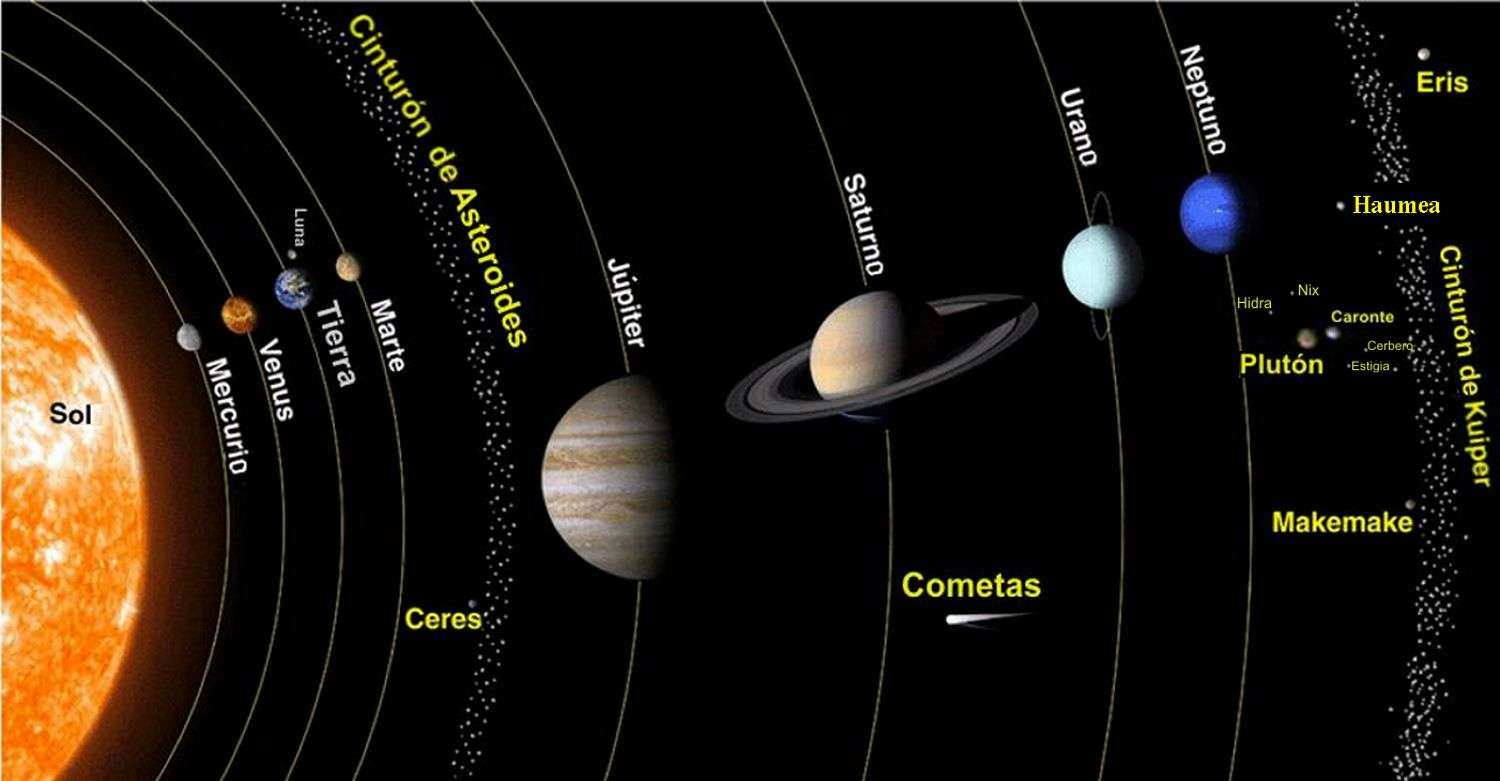
\includegraphics[width=0.8\textwidth]{images/sistema-solar.jpg}
    \caption{Representación del sistema solar.\\Fuente:\url{https://historiaybiografias.com/escala_sistema1/}.}
\end{figure}

La unidad astronómica (AU \textit{en ingles}) es una unidad de longitud que equivale a la distancia media entre la Tierra y el Sol, aproximadamente 150 millones de kilómetros, aunque la Union Astronómica Internacional (IAU) define 1 AU como la longitud igual a 149 597 870 700 metros.   Esta unidad es muy útil para medir distancias en el sistema solar. Por ejemplo, la distancia entre la Tierra y Marte es de aproximadamente 1.5 AU, mientras que la distancia entre la Tierra y Neptuno es de aproximadamente 30 AU.

Utilizando la unidad astronómica como medida de longitud es posible construir un modelo a escala del sistema solar sin que éste ocupe mucho espacio. El diámetro del sol es de 1 392 680 km y en este modelo, el Sol se representaría por una esfera de 30 cm de diámetro, y los planetas se representan por esferas de diferentes tamaños, de acuerdo a su tamaño real.

\textbf{La escala del modelo es de 30 cm = 1 392 680 km.}

Las Efemérides son tablas que contienen información sobre la posición de los cuerpos celestes en el cielo en un momento determinado. En este caso, se utilizarán las efemérides para determinar la posición de los planetas en el sistema solar a una fecha y hora específica.

\section*{Instrucciones}
\begin{enumerate}
    \item Obtener la distancia real en kilómetros del objeto del sistema solar asignado consultando las efemérides en el aplicativo web del JPL de la Nasa, específicamente el valor de \textit{AD: Apoapsis Distance (km)}.
    \item \url{https://ssd.jpl.nasa.gov/horizons/app.html#/}

    \item Suponiendo que (1) el sol tiene un diámetro de 30 cm y que se encuentra ubicado sobre una mesa en el salon 116 del Observatorio Astronómico Nacional y (2) que la orbita del objeto asignado es circular, a ¿qué distancia y qué tamaño tendría el objetivo asignado?
    \begin{itemize}
        \item Grupo 1: Mercurio
        \item Grupo 2: Venus
        \item Grupo 3: Tierra
        \item Grupo 4: Marte
        \item Grupo 5: Júpiter
        \item Grupo 6: Saturno
        \item Grupo 7: Eris
        \item Grupo 8: Urano
        \item Grupo 9: Ceres
        \item Grupo 10: Pluton
        \item Grupo 11: Neptuno
    \end{itemize}
\end{enumerate}

Completar la siguiente tabla:

\begin{table}[htbp]
    \centering
      \begin{tabular}{|r|r|r|r|r|r|}
      \toprule
      \multicolumn{1}{|p{3.07em}|}{Objeto} & \multicolumn{1}{p{8.785em}|}{Distancia real al Sol en millones de km} & \multicolumn{1}{p{7.285em}|}{Distancia real al Sol en AU} & \multicolumn{1}{p{7.715em}|}{Diametro real del objeto en km} & \multicolumn{1}{p{5.355em}|}{Distancia al Sol en m} & \multicolumn{1}{p{3.93em}|}{Diametro en cm} \\
      \midrule
         &    &    &    &    &  \\
      \bottomrule
      \end{tabular}%
    \label{tab:addlabel}%
\end{table}%
  

\begin{enumerate}
    \item Determinar las coordenadas geográficas del falso Sol de 30 cm ubicado en el salon de clase. Sugerencia: usar google-maps para obtener la latitud y la longitud geográficas en decimal. Obtener las coordenadas para el objeto asignado. Deberá ir hasta el lugar para obtener las coordenadas.
\end{enumerate}

Completar la siguiente tabla:
\begin{table}[htbp]
    \centering
      \begin{tabular}{|r|r|r|r|r|}
      \toprule
      \multicolumn{1}{|p{4.215em}|}{Objeto} & \multicolumn{1}{p{5.07em}|}{Latitud geografica (N) del objeto} & \multicolumn{1}{p{5em}|}{Longitud geografica (O) del objeto} & \multicolumn{1}{p{4.785em}|}{Latitud geografica (N) del Sol} & \multicolumn{1}{p{5em}|}{Longitud geografica (O) del Sol} \\
      \midrule
         &    &    &    &  \\
      \bottomrule
      \end{tabular}%
    \label{tab:addlabel}%
\end{table}%

\begin{enumerate}
    \item Introduzca una fotografia del grupo, junto con el objeto asignado y en las coordenadas respectivas en el mapa de google:
    \item \url{https://www.google.com/maps/d/edit?mid=1VVm7JD7jZw56RPK1f9OVQzpc6NzXGKQ&usp=sharing}
    \item Escribir un dato curioso de su objeto:
\end{enumerate}

\end{document}

